\documentclass[conference]{IEEEtran}
\IEEEoverridecommandlockouts

\usepackage{cite}
\usepackage{amsmath,amssymb}
\usepackage{graphicx}
\usepackage{booktabs}
\usepackage{array}
\usepackage{url}
\usepackage{xcolor}
\usepackage{tikz}
\usetikzlibrary{arrows.meta,positioning,calc,fit}
\usepackage{pgfplots}
\pgfplotsset{compat=1.17}

% Generated by prototype/experiments/export_paper_numbers.py; do not edit by hand.
\newcommand{\AccDriveHours}{10.4}
\newcommand{\BaseSerDriveFA}{34.3}
\newcommand{\BaseSerSensFifty}{1.00}
\newcommand{\BaseSerSensFive}{0.46}
\newcommand{\BaseSerSensTen}{0.75}
\newcommand{\BaseSerSensTwenty}{1.00}
\newcommand{\BaseSerSensTwo}{0.34}
\newcommand{\BaseSerWalkFA}{142}
\newcommand{\CardGbAucCardiac}{0.936}
\newcommand{\CardGbAucSeizure}{0.790}
\newcommand{\CardGbRecNormal}{0.93}
\newcommand{\CardGbSzRecords}{6}
\newcommand{\CardLrAucCardiac}{0.955}
\newcommand{\CardLrAucSeizure}{0.846}
\newcommand{\CardLrRecNormal}{0.91}
\newcommand{\CardLrSzRecords}{5}
\newcommand{\CardNbAucCardiac}{0.928}
\newcommand{\CardNbAucSeizure}{0.825}
\newcommand{\CardNbRecNormal}{0.05}
\newcommand{\CardNbSzRecords}{7}
\newcommand{\CycleMax}{57}
\newcommand{\CycleMedian}{2.1}
\newcommand{\CycleP}{3.7}
\newcommand{\DriveHours}{22.2}
\newcommand{\FaFull}{0.09}
\newcommand{\FaNoCam}{0.18}
\newcommand{\FaNoImu}{0.14}
\newcommand{\FaOnlyCard}{3.92}
\newcommand{\FaOnlyMot}{0.00}
\newcommand{\FaOnlyPos}{1.13}
\newcommand{\FaOnlyVis}{0.00}
\newcommand{\FaReal}{0.23}
\newcommand{\FaultCases}{14}
\newcommand{\FaultPassed}{140}
\newcommand{\FaultRuns}{140}
\newcommand{\FaultSeeds}{10}
\newcommand{\FullFalseCount}{2}
\newcommand{\FusionHours}{22.2}
\newcommand{\LatSyFull}{12.0}
\newcommand{\LatSyNoCam}{--}
\newcommand{\LatSyNoImu}{12.0}
\newcommand{\LatSyOnlyCard}{7.5}
\newcommand{\LatSyOnlyMot}{--}
\newcommand{\LatSyOnlyPos}{14.0}
\newcommand{\LatSyOnlyVis}{12.0}
\newcommand{\LatSyReal}{--}
\newcommand{\LatSzFull}{13.2}
\newcommand{\LatSzNoCam}{71.5}
\newcommand{\LatSzNoImu}{15.0}
\newcommand{\LatSzOnlyCard}{30.5}
\newcommand{\LatSzOnlyMot}{--}
\newcommand{\LatSzOnlyPos}{5.2}
\newcommand{\LatSzOnlyVis}{13.0}
\newcommand{\LatSzReal}{78.5}
\newcommand{\MotEpisodes}{324}
\newcommand{\MotGbAuc}{0.857}
\newcommand{\MotGbDriveFA}{4.8}
\newcommand{\MotGbLatTwenty}{2.5}
\newcommand{\MotGbSensFifty}{1.00}
\newcommand{\MotGbSensFive}{0.07}
\newcommand{\MotGbSensTen}{0.91}
\newcommand{\MotGbSensTwenty}{1.00}
\newcommand{\MotGbSensTwo}{0.05}
\newcommand{\MotGbWalkFA}{0.0}
\newcommand{\MotLrAuc}{0.818}
\newcommand{\MotLrDriveFA}{9.2}
\newcommand{\MotLrSensFifty}{1.00}
\newcommand{\MotLrSensFive}{0.34}
\newcommand{\MotLrSensTen}{0.54}
\newcommand{\MotLrSensTwenty}{0.90}
\newcommand{\MotLrSensTwo}{0.24}
\newcommand{\MotLrWalkFA}{3.0}
\newcommand{\MotNbAuc}{0.861}
\newcommand{\MotNbDriveFA}{7.0}
\newcommand{\MotNbSensFifty}{1.00}
\newcommand{\MotNbSensFive}{0.17}
\newcommand{\MotNbSensTen}{0.74}
\newcommand{\MotNbSensTwenty}{1.00}
\newcommand{\MotNbSensTwo}{0.04}
\newcommand{\MotNbWalkFA}{0.0}
\newcommand{\MrCyclingAlarms}{0}
\newcommand{\MrDriveHip}{103}
\newcommand{\MrDriveHipFA}{9.9}
\newcommand{\MrDriveHours}{10.4}
\newcommand{\MrDriveWrist}{48}
\newcommand{\MrDriveWristFA}{4.6}
\newcommand{\MrEpiAuc}{0.98}
\newcommand{\MrEpiHit}{25}
\newcommand{\MrEpiN}{34}
\newcommand{\MrEpiOther}{4}
\newcommand{\MrEpiOtherN}{104}
\newcommand{\MrGaitMaxFA}{35}
\newcommand{\MrHarMax}{23.02}
\newcommand{\MrInjFifty}{0.69}
\newcommand{\MrInjFive}{0.23}
\newcommand{\MrInjTen}{0.25}
\newcommand{\MrInjTwenty}{0.25}
\newcommand{\MrMhAlarms}{3}
\newcommand{\MrMhMin}{110}
\newcommand{\MrNoMhCyclingAlarms}{3}
\newcommand{\MrNoMhDriveHipFA}{5.5}
\newcommand{\MrNoMhDriveWristFA}{2.8}
\newcommand{\MrNoMhMhAlarms}{20}
\newcommand{\MrNoMhRunningAlarms}{17}
\newcommand{\MrNoMhSzAuto}{8/67}
\newcommand{\MrNoMhSzAutoLat}{26}
\newcommand{\MrNoMhSzBgFA}{3.29}
\newcommand{\MrNoMhSzBgHours}{204}
\newcommand{\MrNoMhSzBgPatients}{115}
\newcommand{\MrNoMhSzConv}{44/52}
\newcommand{\MrNoMhSzConvLat}{60}
\newcommand{\MrNoMhSzConvPatients}{36}
\newcommand{\MrNoMhSzHyper}{43/270}
\newcommand{\MrNoMhSzHyperLat}{11}
\newcommand{\MrNoMhSzNonMotor}{17/283}
\newcommand{\MrNoMhSzNonMotorLat}{34}
\newcommand{\MrNoMhSzTonic}{4/29}
\newcommand{\MrNoMhSzTonicLat}{26}
\newcommand{\MrNoMhSzUnclass}{5/97}
\newcommand{\MrNoMhSzUnclassLat}{22}
\newcommand{\MrSzAuto}{20/67}
\newcommand{\MrSzAutoLat}{27}
\newcommand{\MrSzBgFA}{9.08}
\newcommand{\MrSzBgHours}{204}
\newcommand{\MrSzBgPatients}{115}
\newcommand{\MrSzConv}{49/52}
\newcommand{\MrSzConvLat}{52}
\newcommand{\MrSzConvPatients}{36}
\newcommand{\MrSzHyper}{95/270}
\newcommand{\MrSzHyperLat}{10}
\newcommand{\MrSzNonMotor}{40/283}
\newcommand{\MrSzNonMotorLat}{22}
\newcommand{\MrSzTonic}{9/29}
\newcommand{\MrSzTonicLat}{29}
\newcommand{\MrSzUnclass}{18/97}
\newcommand{\MrSzUnclassLat}{18}
\newcommand{\NSyncopeEp}{80}
\newcommand{\NcardCardiac}{2{,}521}
\newcommand{\NcardNormal}{51{,}003}
\newcommand{\NcardRecords}{130}
\newcommand{\NcardSeizure}{166}
\newcommand{\PctSyFull}{14.1}
\newcommand{\PctSzFull}{28.3}
\newcommand{\SweepFullEight}{0.00}
\newcommand{\SweepFullFour}{0.05}
\newcommand{\SweepFullTwo}{0.09}
\newcommand{\SweepFullZero}{0.00}
\newcommand{\SweepLatEight}{16.5}
\newcommand{\SweepLatFour}{13.5}
\newcommand{\SweepLatTwo}{12.0}
\newcommand{\SweepLatZero}{11.5}
\newcommand{\SweepRealEight}{0.05}
\newcommand{\SweepRealFour}{0.14}
\newcommand{\SweepRealTwo}{0.23}
\newcommand{\SweepRealZero}{0.14}
\newcommand{\SyFull}{79/80}
\newcommand{\SyNoCam}{0/80}
\newcommand{\SyNoImu}{79/80}
\newcommand{\SyOnlyCard}{47/80}
\newcommand{\SyOnlyMot}{0/80}
\newcommand{\SyOnlyPos}{79/80}
\newcommand{\SyOnlyVis}{80/80}
\newcommand{\SyReal}{0/80}
\newcommand{\SzFull}{10/10}
\newcommand{\SzFullFifty}{10/10}
\newcommand{\SzFullTen}{9/10}
\newcommand{\SzFullTwenty}{10/10}
\newcommand{\SzMimFull}{10/10}
\newcommand{\SzMimNoCam}{10/10}
\newcommand{\SzMimNoImu}{9/10}
\newcommand{\SzMimOnlyCard}{5/10}
\newcommand{\SzMimOnlyMot}{10/10}
\newcommand{\SzMimOnlyPos}{10/10}
\newcommand{\SzMimOnlyVis}{10/10}
\newcommand{\SzMimReal}{8/10}
\newcommand{\SzModFull}{29/30}
\newcommand{\SzModNoCam}{15/30}
\newcommand{\SzModNoImu}{28/30}
\newcommand{\SzModOnlyCard}{15/30}
\newcommand{\SzModOnlyMot}{0/30}
\newcommand{\SzModOnlyPos}{30/30}
\newcommand{\SzModOnlyVis}{30/30}
\newcommand{\SzModReal}{6/30}
\newcommand{\SzNoCam}{4/10}
\newcommand{\SzNoImu}{10/10}
\newcommand{\SzOnlyCard}{5/10}
\newcommand{\SzOnlyMot}{0/10}
\newcommand{\SzOnlyPos}{10/10}
\newcommand{\SzOnlyVis}{10/10}
\newcommand{\SzReal}{2/10}
\newcommand{\SzRecords}{7}
\newcommand{\WrongFull}{0}
\newcommand{\WrongNoCam}{0}
\newcommand{\WrongNoImu}{0}
\newcommand{\WrongOnlyCard}{0}
\newcommand{\WrongOnlyMot}{0}
\newcommand{\WrongOnlyPos}{1}
\newcommand{\WrongOnlyVis}{0}
\newcommand{\WrongReal}{0}

% Generated by prototype/experiments/export_paper_numbers.py from results/external_checks.json.
\newcommand{\EpiN}{34}
\newcommand{\EpiOtherN}{104}
\newcommand{\EpiTransferHit}{3}
\newcommand{\EpiTransferOther}{1}
\newcommand{\EpiWithinHit}{33}
\newcommand{\EpiWithinOther}{0}
\newcommand{\HarMaxRate}{0.8}
\newcommand{\MhCyclingAlarms}{10}
\newcommand{\MhCyclingMin}{10}
\newcommand{\MhOtherAlarms}{0}
\newcommand{\MhWalkingAlarms}{4}


\begin{document}

\title{CabinGuard-ADI: Bounded-Evidence Multimodal Detection of Acute Driver Incapacitation with an Authenticated Minimum-Risk Response\thanks{Submitted to the IEEE VTS TSYP14 CabinGuard-ADI Technical Challenge, Phase 1. Code, trained models and every result file accompany the submission.}}

% Phase 1 review is anonymous: no names, affiliations or e-mail addresses.
\author{\IEEEauthorblockN{Anonymous Authors}
\IEEEauthorblockA{Affiliation withheld for review}}

\maketitle

\begin{abstract}
Driver monitoring systems detect drowsiness and distraction, not the sudden loss of driving capacity caused by cardiac syncope or a convulsive seizure. CabinGuard-ADI separates these two events from normal driving using four contactless channels: camera pulse rhythm, eyelid and head pose, a headrest accelerometer, and seat and steering-wheel sensors. The evidence of every channel is bounded so that no single sensor can trigger a vehicle response; a minimum-risk manoeuvre needs two physical sensors that agree for 2 seconds. The pulse-rhythm and motion branches are trained on public PhysioNet recordings, including \DriveHours\ hours of road driving, ten annotated seizures, ventricular arrhythmia onsets and \AccDriveHours\ hours of driving accelerometry, and are evaluated across held-out records and subjects. On out-of-fold composite episodes the fused detector started no manoeuvre in \FusionHours\ hours of real driving, a 95\,\% upper bound of \FaFullUpper\ per hour, against \FaOnlyCard\ false starts per hour for the pulse branch alone, and detected \SyFull\ syncope and \SzFull\ seizure episodes with median latencies of \LatSyFull\ and \LatSzFull\ seconds from onset. The manoeuvre is commanded through authenticated CAN frames and supervised by a gateway that rejects forged, replayed and implausible commands and completes the stop if the detector fails. A signed and encrypted 76-byte medical extension reaches the emergency centre, while nearby vehicles are warned without the diagnosis. The eye, head and seat channels still use modelled likelihoods, and a motion branch trained on injected seizure motion detected few recorded seizure mimics; the Phase 2 bench replaces both with measured signals.
\end{abstract}

\begin{IEEEkeywords}
Driver monitoring, driver incapacitation, syncope, epileptic seizure, multimodal fusion, remote photoplethysmography, minimum risk manoeuvre, SecOC, eCall
\end{IEEEkeywords}

\section{Introduction and Motivation}
Sudden illness of the driver is a small but persistent cause of fatal crashes: in Finland and in the Swiss canton of Vaud it caused 1.5\,\% and 3.4\,\% of all traffic deaths, and probable cardiac arrest alone about 2\,\% of driver deaths~\cite{halinen1994}. Since July 2022 new European vehicles must carry drowsiness and distraction warning systems, and the same regulation requires those systems to work without biometric information~\cite{eu2019gsr}. Neither function addresses a driver who loses consciousness or motor control within seconds.

Two events dominate that scenario. Cardiac syncope is a transient loss of consciousness from cerebral hypoperfusion caused by an arrhythmia~\cite{shen2017}; the driver becomes flaccid, the head drops and the hands leave the wheel. A convulsive seizure begins with a tonic phase of sustained contraction and continues with clonic, rhythmic jerking~\cite{fisher2017}. The two look different only on average: myoclonic jerks occurred in 90\,\% of syncopes induced in healthy volunteers~\cite{lempert1994}, so a motion sensor alone confuses them, while a camera alone cannot tell closed eyes from a blinded lens. An unnecessary manoeuvre on a motorway is itself a hazard.

The contributions are a fusion rule under which no single sensor can start a manoeuvre, with the bound derived from the decision threshold; pulse-rhythm and motion detectors evaluated on public real recordings, including real road driving; a gateway that accepts only authenticated, plausible commands and fails safe; and an emergency message that gives the etiology to the emergency centre alone.

\section{Related Work}
Camera-based pulse measurement projects the skin colour signal onto a plane orthogonal to the skin tone (POS)~\cite{wang2017pos}; in a moving car, narrow-band near-infrared video reduces the effect of changing daylight~\cite{nowara2022}. Real-road driver ECG comes from the driver-stress study of Healey and Picard~\cite{healey2005}, and eye closure is commonly measured with the eye aspect ratio~\cite{soukupova2016}.

Seizure detection outside hospitals relies mostly on wearables: a wrist accelerometer detected 35 of 39 generalized tonic-clonic seizures with 0.2 false alarms per day~\cite{beniczky2013}. Clonic discharges last about 0.2\,s with silent periods of exponentially increasing duration~\cite{conradsen2013}, and heart rate rises during most partial seizures~\cite{alaweel1999}; none of these studies measures motion through a vehicle seat.

On the vehicle side, UN Regulation No.~157 defines a minimum risk manoeuvre that an automated lane keeping system performs when a transition demand is not answered~\cite{unece157}. In-vehicle networks without authentication let a compromised node command brakes~\cite{koscher2010}, cameras can be blinded with commodity lasers~\cite{petit2015}, and AUTOSAR secure onboard communication (SecOC) adds truncated message authentication codes and freshness values to CAN frames~\cite{autosar_secoc}.

\section{Problem Definition}
Every 100\,ms the system assigns the driver to a class $C\in\{\mathrm{N},\mathrm{S},\mathrm{Z}\}$ for normal driving, cardiac syncope and convulsive seizure, and decides whether to start a minimum risk manoeuvre (MRM). It must meet five requirements: R1, few false MRM starts per hour of normal driving; R2, detection within seconds of onset; R3, no single sensor able to start an MRM; R4, safe behaviour under sensor, processing and communication failure and under tampered or unauthorized messages; R5, only the minimum necessary data leaving the vehicle. A false start first produces a 3\,s alert that a conscious driver cancels, so R1 counts alerts as well as braking.

\section{System Architecture}
The sensing layer has three physical sensors, shown on the left of Fig.~\ref{fig:arch}. A 30\,fps camera with 850\,nm illumination on the steering column yields the pulse beat times, the eye aspect ratio $e$ and the head pitch $\theta$. An MPU6050 accelerometer in the headrest is sampled at 100\,Hz. A force-sensing resistor in the seatback, a second one in the wheel rim, two capacitive touch pads and the steering torque $\tau$ form the seat and wheel sensor. An ESP32 node streams these signals in 24-byte frames with a sequence number and CRC to the edge host, which runs detection, the watchdog and the MRM state machine and commands the vehicle only through one authenticated CAN message to a gateway that owns the actuators. Every input carries a timestamp, and data older than 300\,ms is treated as missing.

\begin{figure*}[!t]
\centering
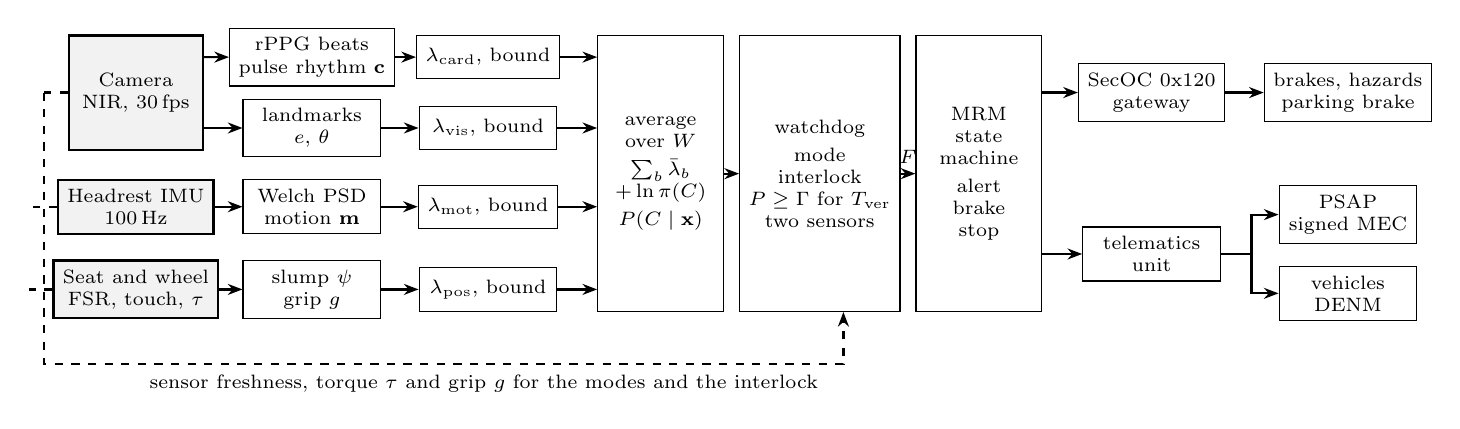
\begin{tikzpicture}[x=0.86cm,
  font=\scriptsize, >={Stealth[scale=0.8]},
  sen/.style={draw, thick, minimum width=1.7cm, minimum height=0.55cm, align=center, fill=black!5},
  box/.style={draw, minimum width=1.75cm, minimum height=0.55cm, align=center},
  arr/.style={->, thick}]
  \node[sen, minimum height=1.45cm] (cam) at (0,3.0) {Camera\\NIR, 30\,fps};
  \node[sen] (imu) at (0,1.55) {Headrest IMU\\100\,Hz};
  \node[sen] (seat) at (0,0.5) {Seat and wheel\\FSR, touch, $\tau$};
  \node[box] (fc) at (2.6,3.45) {rPPG beats\\pulse rhythm $\mathbf{c}$};
  \node[box] (fv) at (2.6,2.55) {landmarks\\$e$, $\theta$};
  \node[box] (fm) at (2.6,1.55) {Welch PSD\\motion $\mathbf{m}$};
  \node[box] (fp) at (2.6,0.5) {slump $\psi$\\grip $g$};
  \node[box] (bc) at (5.2,3.45) {$\lambda_{\mathrm{card}}$, bound};
  \node[box] (bv) at (5.2,2.55) {$\lambda_{\mathrm{vis}}$, bound};
  \node[box] (bm) at (5.2,1.55) {$\lambda_{\mathrm{mot}}$, bound};
  \node[box] (bp) at (5.2,0.5) {$\lambda_{\mathrm{pos}}$, bound};
  \node[box, minimum height=3.5cm, minimum width=1.6cm] (fu) at (7.75,1.97) {average\\over $W$\\[2pt]$\sum_b\bar\lambda_b$\\$+\ln\pi(C)$\\[2pt]$P(C\mid\mathbf{x})$};
  \node[box, minimum height=3.5cm, minimum width=2.0cm] (wd) at (10.1,1.97) {watchdog\\[2pt]mode\\interlock\\$P\ge\Gamma$ for $T_{\mathrm{ver}}$\\two sensors};
  \node[box, minimum height=3.5cm, minimum width=1.6cm] (sm) at (12.45,1.97) {MRM\\state\\machine\\[2pt]alert\\brake\\stop};
  \node[box] (gw) at (15.0,3.0) {SecOC 0x120\\gateway};
  \node[box] (act) at (17.9,3.0) {brakes, hazards\\parking brake};
  \node[box] (tel) at (15.0,0.95) {telematics\\unit};
  \node[box] (psap) at (17.9,1.45) {PSAP\\signed MEC};
  \node[box] (v2x) at (17.9,0.45) {vehicles\\DENM};
  \draw[arr] ([yshift=0.45cm]cam.east) -- (fc.west);
  \draw[arr] ([yshift=-0.45cm]cam.east) -- (fv.west);
  \draw[arr] (imu) -- (fm);
  \draw[arr] (seat) -- (fp);
  \draw[arr] (fc) -- (bc); \draw[arr] (fv) -- (bv); \draw[arr] (fm) -- (bm); \draw[arr] (fp) -- (bp);
  \draw[arr] (bc.east) -- (bc.east -| fu.west);
  \draw[arr] (bv.east) -- (bv.east -| fu.west);
  \draw[arr] (bm.east) -- (bm.east -| fu.west);
  \draw[arr] (bp.east) -- (bp.east -| fu.west);
  \draw[arr] (fu) -- (wd);
  \draw[arr] (wd) -- node[above]{$F$} (sm);
  \draw[arr] (sm.east |- gw.west) -- (gw.west);
  \draw[arr] (sm.east |- tel.west) -- (tel.west);
  \draw[arr] (gw) -- (act);
  \draw[arr] (tel.east) -- ++(0.45,0) |- (psap.west);
  \draw[arr] (tel.east) -- ++(0.45,0) |- (v2x.west);
  \draw[thick, dashed] (cam.west) -- ++(-0.35,0) coordinate (h1);
  \draw[thick, dashed] (imu.west) -- ++(-0.35,0);
  \draw[thick, dashed] (seat.west) -- ++(-0.35,0);
  \draw[arr, dashed] (h1) -- ++(0,-3.45) -- node[pos=0.55, below]{sensor freshness, torque $\tau$ and grip $g$ for the modes and the interlock} ([xshift=0.3cm]wd.south |- 0,-0.45) -- ([xshift=0.3cm]wd.south);
\end{tikzpicture}
\caption{CabinGuard-ADI signal flow from the three sensors to the vehicle actuators and the two emergency receivers.}
\label{fig:arch}
\end{figure*}

\section{Detection Methodology}
\subsection{Features}
The camera front end detects pulse peaks in the POS signal~\cite{wang2017pos}; in the public recordings used for training the beats are ECG R-peaks instead. Over a 10\,s window the pulse-rhythm vector $\mathbf{c}$ holds the rate from the median inter-beat interval, its difference from the driver's own running baseline, the coefficient of variation of the intervals, and the fraction $a$ of the window not covered by intervals shorter than 2\,s. Ventricular fibrillation, flutter and asystole produce no pulse, so they raise $a$ towards one. Eye opening is the eye aspect ratio of Soukupov\'a and \v{C}ech~\cite{soukupova2016}, computed from six eyelid landmarks.
\begin{equation}
e=\frac{\lVert p_2-p_6\rVert+\lVert p_3-p_5\rVert}{2\,\lVert p_1-p_4\rVert}
\label{eq:ear}
\end{equation}
In Equation~\eqref{eq:ear}, $p_1$ and $p_4$ are the eye corners and $p_2,p_3,p_5,p_6$ the upper and lower lid points in image coordinates. Clonic motion is characterised by the share of acceleration power in the 2--6\,Hz band, computed over a 2\,s window from the sum $S(f)$ of the three per-axis Welch spectra~\cite{welch1967}.
\begin{equation}
r=\frac{\int_{2}^{6}S(f)\,\mathrm{d}f}{\int_{0.5}^{20}S(f)\,\mathrm{d}f}
\label{eq:ser}
\end{equation}
In Equation~\eqref{eq:ser}, $r$ is the spectral energy ratio and $f$ the frequency in hertz. A ratio alone is noisy when the body is still, so the motion vector $\mathbf{m}$ adds the 2--6\,Hz RMS acceleration, the peak frequency, the total RMS, the largest autocorrelation at lags of 0.15--0.5\,s, which captures the repetition of jerks, and the peak-to-mean ratio of the band spectrum. Postural slump $\psi$ is one minus the mean normalized seatback pressure over 1\,s, and $g$ is the grip state: active, disengaged, or clenched when the rim force exceeds a threshold.

\subsection{Branch Evidence}
Four branches turn features into evidence. The cardiac branch is a multinomial logistic regression on $\mathbf{c}$ and the motion branch gradient-boosted trees~\cite{friedman2001} with histogram splits~\cite{ke2017} on $\mathbf{m}$, both trained with class weights that balance the classes. The vision branch on $(e,\theta)$ and the posture branch on $(\psi,g)$ use expert-set Gaussian and categorical class densities, since no public recording provides them for incapacitated drivers. A discriminative model's posterior becomes a likelihood ratio once its training prior is divided out, the scaled-likelihood step of hybrid connectionist recognisers~\cite{bourlard1994}.
\begin{equation}
\lambda_b(C)=\ln\frac{P_b(C\mid\mathbf{x}_b)}{\pi_b(C)}-\ln\frac{P_b(\mathrm{N}\mid\mathbf{x}_b)}{\pi_b(\mathrm{N})}
\label{eq:llr}
\end{equation}
In Equation~\eqref{eq:llr}, $\lambda_b(C)$ is the log-likelihood ratio of class $C$ against normal driving from branch $b$, $\mathbf{x}_b$ the branch input and $\pi_b$ the prior the model was trained under, uniform here because of the balanced weights. The motion branch only separates clonic motion from everything else, so it gives $\lambda_{\mathrm{mot}}(\mathrm{S})=0$.

\subsection{Bounded-Evidence Fusion}
Each branch's evidence for an event is limited to a bound $c$ by shifting both event classes together, which keeps the branch's preference between syncope and seizure.
\begin{equation}
\tilde\lambda_b(C)=\max\Bigl(-c,\;\lambda_b(C)-\max\bigl(0,\max_{C'\neq\mathrm{N}}\lambda_b(C')-c\bigr)\Bigr)
\label{eq:bound}
\end{equation}
In Equation~\eqref{eq:bound}, $\tilde\lambda_b(C)$ is the bounded evidence for $C\neq\mathrm{N}$ and $C'$ ranges over the two event classes. Treating the branches as conditionally independent given the class, the product rule for combining classifiers~\cite{kittler1998} gives the fused posterior.
\begin{equation}
P(C\mid\mathbf{x})\propto\pi(C)\exp\Bigl(\sum_{b\in\mathcal{A}}\bar\lambda_b(C)\Bigr)
\label{eq:fusion}
\end{equation}
In Equation~\eqref{eq:fusion}, $\mathcal{A}$ is the set of branches whose sensors are available, $\bar\lambda_b$ the average of $\tilde\lambda_b$ over the last $W=2$\,s, and $\pi$ the operational prior with $\pi(\mathrm{N})=0.8$ and $0.1$ for each event. With the decision threshold $\Gamma=0.85$ and the prior log-odds $l_0=\ln(0.1/0.8)$, the bound is chosen so that one branch cannot reach $\Gamma$ while two agreeing branches can.
\begin{equation}
l_0+c<\ln\frac{\Gamma}{1-\Gamma}<l_0+2c
\label{eq:cap}
\end{equation}
Equation~\eqref{eq:cap} holds for $1.91<c<3.81$, and $c=3$ is used. A missing branch simply leaves the sum in Equation~\eqref{eq:fusion}, so sensor loss never needs a separate model.

\subsection{Decision Rule}
The watchdog sets the flag $F$ that starts the MRM when one event class keeps $P(C\mid\mathbf{x})\ge\Gamma$ for $T_{\mathrm{ver}}=2$\,s and at least two physical sensors give $\bar\lambda_b(C)\ge1$. The camera feeds two branches but counts as one sensor, so a blinded lens reporting closed eyes and no pulse cannot decide alone.

\section{Safety Response and Fault Handling}
Once $F$ is set, the state machine follows the transition-demand sequence of UN Regulation No.~157~\cite{unece157} with design values of our own: a 3\,s audible and haptic alert that the driver cancels by braking or by more than 4\,Nm of steering torque, unless the torque coincides with clonic motion or a clenched grip; hazard lights and escalation; braking at $-3.2$\,m/s$^2$ from 10\,s after the alert with a lateral move to the shoulder; and at standstill the parking brake and door unlock. The emergency call is placed when the alert goes unanswered, not after the stop.

The watchdog derives the mode from sensor freshness. Losing the camera removes the cardiac and vision branches (degraded mode 1), losing the accelerometer removes the motion branch (degraded mode 2), and with fewer than two sensors left no MRM may start and the driver is warned instead (degraded mode 3). When the camera reports no pulse or closed eyes while the wheel shows an upright driver steering with more than 1\,Nm, the readings contradict each other, so the camera is distrusted for 10\,s and the event is logged.

The gateway trusts no command. A frame must pass authentication and a plausibility gate that allows only the phase order of the state machine and decelerations between 0 and $-4$\,m/s$^2$. The command doubles as an alive signal: after 300\,ms without a valid frame the gateway flags an ECU fault and, if the driver is still in control, actuates nothing; if a manoeuvre is already under way it completes the stop, because a driver judged incapacitated cannot take over. The host itself goes silent after three consecutive 100\,ms deadline overruns. The emergency message is retried with 1, 2 and 4\,s backoff on the cellular bearer, then sent by SMS, and otherwise kept and retried every 30\,s; the manoeuvre never waits for it.

\section{Cybersecurity and Threat Model}
The protected assets are the vehicle actuators, the driver's physiological data, the integrity of the emergency message and the driver's identity and location. The sensor link inside the cabin is protected against corruption by its CRC but not against an attacker with physical access, which is outside the scope; the CAN bus, the cellular network and the radio channel are untrusted, and the gateway is the trusted boundary in front of the actuators. Table~\ref{tab:threats} lists the threats and the control that answers each.

\begin{table}[!t]
\caption{Threats, controls and the fault-matrix case that exercises each}
\label{tab:threats}
\centering
\footnotesize
\begin{tabular}{@{}>{\raggedright\arraybackslash}p{2.15cm}>{\raggedright\arraybackslash}p{3.35cm}>{\raggedright\arraybackslash}p{2.1cm}@{}}
\toprule
Threat & Control & Test case \\
\midrule
Forged command & 24-bit AES-CMAC, SecOC profile 1 & unauthorized key \\
Replayed command & 64-bit freshness counter, 8 bits sent & replayed frames \\
Tampered frame & MAC check, alive timeout & tampered frames \\
Valid MAC, unsafe value & phase order, $-4$\,m/s$^2$ limit & implausible command \\
Camera blinding or spoofing & cross-sensor interlock, two-sensor rule & optical blinding \\
Sensor loss or stale data & freshness, degraded modes & IMU, seat stale \\
ECU hang & fail-silent host, gateway takeover & two processing cases \\
Network outage & retry, SMS fallback, queue & two bearer cases \\
Message forgery, eavesdropping & ECDSA P-256 signature, ECIES to PSAP & unit tests \\
\bottomrule
\end{tabular}
\end{table}

The 0x120 command follows SecOC profile 1, AES-128-CMAC~\cite{nist80038b} truncated to 24 bits over the data identifier, payload and a 64-bit freshness value of which the low 8 bits are sent~\cite{autosar_secoc}. Its payload, the CAN database file and the decoder are tested to agree bit for bit. The status frame that other nodes can read carries sensor health only, never a biometric value.

The 76-byte medical extension container (MEC) has a 12-byte header (version, etiology, confidence, detection latency, sensor mask, heart rate, sequence number, timestamp) and a 64-byte ECDSA P-256 signature from a pseudonymous key, the curve and signature used by ITS security certificates~\cite{etsi103097}. It is encrypted to the emergency centre's public key with ephemeral ECDH, HKDF and AES-GCM and fits as optional additional data next to the 140-byte eCall minimum set of data~\cite{en15722}, which already carries the location. Nearby vehicles receive a decentralized environmental notification with cause code 93, human problem, and sub-cause 0, unavailable~\cite{etsi102894}, so the etiology never leaves the emergency channel. The system stores no video and no waveform; only 10\,s feature buffers exist, in memory.

\section{Evaluation Methodology}
Table~\ref{tab:data} lists the public recordings, all from PhysioNet~\cite{goldberger2000}. Driving-study R-peaks come from the WFDB XQRS detector. Windows in VT are labelled cardiac and keep their beats; windows in fibrillation, flutter or asystole are labelled cardiac and lose their beats, because no pulse reaches the face. Atrial fibrillation, bigeminy and other rhythms that do not incapacitate count as normal, as hard negatives.

\begin{table}[!t]
\caption{Public recordings used for training and evaluation}
\label{tab:data}
\centering
\footnotesize
\begin{tabular}{@{}>{\raggedright\arraybackslash}p{2.9cm}>{\raggedright\arraybackslash}p{2.35cm}>{\raggedright\arraybackslash}p{2.4cm}@{}}
\toprule
Database & Content & Role \\
\midrule
Driver stress~\cite{healey2005} & ECG, 17 road drives & normal, \DriveHours\,h \\
Partial epilepsy~\cite{alaweel1999} & ECG, 10 seizures & seizure, normal \\
Malignant ventricular ectopy~\cite{greenwald1986} & ECG, 22 records & syncope, normal \\
CU tachyarrhythmia~\cite{nolle1986} & ECG, 35 records & syncope, normal \\
MIT-BIH arrhythmia~\cite{moody2001} & ECG, 48 records & syncope, normal \\
Walk, climb, drive~\cite{karas2021} & 100\,Hz accel., 32 adults & motion, \AccDriveHours\,h driving \\
\bottomrule
\end{tabular}
\end{table}

Branches are evaluated with leave-one-record-out validation for the cardiac branch (\NcardRecords\ records) and leave-one-subject-out validation for the motion branch, using the hip accelerometer as the closest available proxy for a seat-mounted sensor. No public recording measures seizure motion in a seat, so motion positives are real driving windows with an added jerk train that follows the clonic dynamics of~\cite{conradsen2013}: 0.2\,s discharges with silent periods starting at 0.05--0.15\,s and growing to about 1\,s over 40 jerks, at amplitudes of 0.02 to 0.5\,g. Only amplitudes of 0.1\,g and above are used as training positives; all are scored.

The fused detector is evaluated on composite episodes, which is the conditional-independence assumption of Equation~\eqref{eq:fusion} applied to the test data. A normal episode pairs a whole held-out drive with held-out driving accelerometry. A syncope episode takes \NSyncopeEp\ ventricular arrhythmia onsets with 30\,s of normal rhythm before them; loss of consciousness, which drives the vision and posture channels, follows after 6--12\,s, an assumption. A seizure episode takes each of the ten seizures, a 5--15\,s tonic phase and then injected clonic motion at 0.1, 0.2 and 0.5\,g. Vision and posture channels are generated with everyday confounders: blinks, 1--3\,s glances down every 45\,s, forward leans every 120\,s and one-handed steering every 60\,s. Every model is applied out of fold. Two further checks use recordings downloaded outside the main pipeline: seizure mimics performed by healthy volunteers with a wrist accelerometer at 16\,Hz~\cite{villar2016}, and everyday activities from a chest sensor~\cite{banos2014} and a waist-worn phone~\cite{anguita2013}. The deployed motion branch is applied unchanged after resampling to 100\,Hz, and, as a reference, the same features are trained on the mimic dataset's own training split. Separately, the full software pipeline runs \FaultCases\ failure and attack cases with synthetic sensors, \FaultSeeds\ seeds each.

\section{Results}
Table~\ref{tab:branch} gives the branch results. The pulse rhythm separates ventricular arrhythmia well and seizures less well, which matches ictal heart-rate rises of 3 to 88\,bpm in this database~\cite{alaweel1999}. The fixed spectral-ratio rule $r>0.65$ fires \BaseSerDriveFA\ times per hour of real driving, so road vibration alone defeats it, and its higher sensitivity to weak injected jerks (\BaseSerSensFive\ against \MotGbSensFive\ at 0.05\,g) comes only from that; the learned motion branch reduces the rate to \MotGbDriveFA\ per hour, still too many for a standalone trigger.

\begin{table}[!t]
\caption{Branch results under held-out records and held-out subjects}
\label{tab:branch}
\centering
\footnotesize
\begin{tabular}{@{}lccc@{}}
\toprule
Cardiac branch & Gaussian NB & Logistic & Boosted trees \\
\midrule
AUC, VT/VF vs rest & \CardNbAucCardiac & \CardLrAucCardiac & \CardGbAucCardiac \\
AUC, seizure vs rest & \CardNbAucSeizure & \CardLrAucSeizure & \CardGbAucSeizure \\
Seizure records hit, of \SzRecords & \CardNbSzRecords & \CardLrSzRecords & \CardGbSzRecords \\
\midrule
Motion branch & Gaussian NB & Logistic & Boosted trees \\
\midrule
AUC, driving vs clonic & \MotNbAuc & \MotLrAuc & \MotGbAuc \\
Alarms per driving hour & \MotNbDriveFA & \MotLrDriveFA & \MotGbDriveFA \\
Sensitivity at 0.05\,g & \MotNbSensFive & \MotLrSensFive & \MotGbSensFive \\
Sensitivity at 0.1\,g & \MotNbSensTen & \MotLrSensTen & \MotGbSensTen \\
Sensitivity at 0.2\,g & \MotNbSensTwenty & \MotLrSensTwenty & \MotGbSensTwenty \\
\bottomrule
\end{tabular}
\end{table}

The deployed models are the logistic cardiac branch and the boosted-tree motion branch, each the best of the three on its own evaluation. Table~\ref{tab:fusion} shows what fusion adds. Only the cardiac and motion rows are scored on real signals; the vision and posture channels are generated from the same expert densities that score them, so their near-perfect rows are circular and every row that includes them inherits part of that optimism. On real signals alone, the cardiac branch raises \FaOnlyCard\ false starts per hour, and adding the motion branch cuts this to \FaReal\ but cannot confirm syncope, which the motion branch says nothing about. All four branches started no manoeuvre in \FusionHours\ hours of real driving, which puts the 95\,\% upper bound of the rate at \FaFullUpper\ per hour, and detected \SyFull\ syncope and \SzFull\ seizure episodes with 90th-percentile latencies of \PctSyFull\ and \PctSzFull\,s from onset. Losing the camera keeps seizure detection but, by design, confirms no syncope, since only the seat would still support it.

\begin{table}[!t]
\caption{Fused detector on out-of-fold composite episodes}
\label{tab:fusion}
\centering
\footnotesize
\begin{tabular}{@{}lcccc@{}}
\toprule
Branches & False/h & Syncope & Seizure & Latency, s \\
\midrule
Cardiac only & \FaOnlyCard & \SyOnlyCard & \SzOnlyCard & \LatSyOnlyCard, \LatSzOnlyCard \\
Motion only & \FaOnlyMot & \SyOnlyMot & \SzOnlyMot & \LatSyOnlyMot, \LatSzOnlyMot \\
Vision only & \FaOnlyVis & \SyOnlyVis & \SzOnlyVis & \LatSyOnlyVis, \LatSzOnlyVis \\
Posture only & \FaOnlyPos & \SyOnlyPos & \SzOnlyPos & \LatSyOnlyPos, \LatSzOnlyPos \\
Cardiac, motion & \FaReal & \SyReal & \SzReal & \LatSyReal, \LatSzReal \\
All four & \FaFull & \SyFull & \SzFull & \LatSyFull, \LatSzFull \\
Camera lost & \FaNoCam & \SyNoCam & \SzNoCam & \LatSyNoCam, \LatSzNoCam \\
IMU lost & \FaNoImu & \SyNoImu & \SzNoImu & \LatSyNoImu, \LatSzNoImu \\
\bottomrule
\end{tabular}
\end{table}

The averaging window $W$ was searched over 0, 2, 4 and 8\,s on these same episodes. The fused detector started no manoeuvre at any of them, and the median syncope latency grew from \SweepLatZero\ to \SweepLatEight\,s; $W=2$\,s is the shortest window with the highest syncope sensitivity, a choice made on the test episodes and therefore optimistic.

The recorded seizure mimics expose the limit of training on injected motion. The deployed branch fired on only \EpiTransferHit\ of \EpiN\ mimics, and on \EpiTransferOther\ of \EpiOtherN\ walking, running and sawing recordings; the same features trained on the mimic dataset fired on \EpiWithinHit\ of \EpiN\ mimics and \EpiWithinOther\ of the others. The features carry the information, but the seizure sensitivities of Table~\ref{tab:fusion} hold only for motion that resembles the injection model. On everyday activities the branch alone raised \MhCyclingAlarms\ alarms in \MhCyclingMin\,min of cycling and \MhWalkingAlarms\ during walking, none in the other activities, and flagged at most \HarMaxRate\,\% of phone windows, which leaves the two-sensor rule to absorb rhythmic movement.


All \FaultPassed\ of \FaultRuns\ fault-matrix runs reached the required outcome: no manoeuvre under sensor loss, stale data, optical blinding, or tampered, replayed, forged or implausible commands; a fail-silent gateway when the host hangs during normal driving and a completed stop when it hangs during a manoeuvre; and a delivered, verified MEC after cellular loss or a 60\,s loss of every bearer. On one laptop core the detection cycle took \CycleMedian\,ms at the median and \CycleP\,ms at the 99th percentile; the slowest of all cycles took \CycleMax\,ms, which the three-overrun rule tolerates.

\section{Conclusion}
Bounding each sensor's evidence and requiring two physical sensors made the detector both sensitive and quiet on real driving, and the vehicle moves only on commands that a fail-safe gateway authenticates. Three limits remain. The vision and posture likelihoods are expert-set and their channels modelled, so the fused results above are an upper estimate until those channels are measured; seizure motion is injected rather than measured in a seat, and the branch trained on it misses most recorded seizure mimics until it is retrained on such recordings; and the composite episodes assume that the branches are independent given the class. The same code already runs on an ESP32 sensor node, a camera and a CAN bus; Phase 2 volunteer sessions on that bench will measure the eye, head and seat likelihoods, the seizure-mimic amplitude at the headrest, camera pulse accuracy and timing on the target processor.

\begin{thebibliography}{00}
\bibitem{halinen1994} M.~O. Halinen and A.~Jaussi, ``Fatal road accidents caused by sudden death of the driver in Finland and Vaud, Switzerland,'' \emph{Eur. Heart J.}, vol.~15, no.~7, pp.~888--894, 1994.
\bibitem{eu2019gsr} ``Regulation (EU) 2019/2144 on type-approval requirements for motor vehicles as regards their general safety,'' \emph{Off. J. Eur. Union}, L 325, Dec. 2019.
\bibitem{shen2017} W.-K. Shen \emph{et al.}, ``2017 ACC/AHA/HRS guideline for the evaluation and management of patients with syncope,'' \emph{Circulation}, vol.~136, no.~5, pp.~e25--e59, 2017.
\bibitem{fisher2017} R.~S. Fisher \emph{et al.}, ``Operational classification of seizure types by the International League Against Epilepsy,'' \emph{Epilepsia}, vol.~58, no.~4, pp.~522--530, 2017.
\bibitem{lempert1994} T.~Lempert, M.~Bauer, and D.~Schmidt, ``Syncope: A videometric analysis of 56 episodes of transient cerebral hypoxia,'' \emph{Ann. Neurol.}, vol.~36, no.~2, pp.~233--237, 1994.
\bibitem{wang2017pos} W.~Wang, A.~C. den Brinker, S.~Stuijk, and G.~de Haan, ``Algorithmic principles of remote PPG,'' \emph{IEEE Trans. Biomed. Eng.}, vol.~64, no.~7, pp.~1479--1491, 2017.
\bibitem{nowara2022} E.~M. Nowara, T.~K. Marks, H.~Mansour, and A.~Veeraraghavan, ``Near-infrared imaging photoplethysmography during driving,'' \emph{IEEE Trans. Intell. Transp. Syst.}, vol.~23, no.~4, 2022.
\bibitem{healey2005} J.~A. Healey and R.~W. Picard, ``Detecting stress during real-world driving tasks using physiological sensors,'' \emph{IEEE Trans. Intell. Transp. Syst.}, vol.~6, no.~2, pp.~156--166, 2005.
\bibitem{soukupova2016} T.~Soukupov\'a and J.~\v{C}ech, ``Real-time eye blink detection using facial landmarks,'' in \emph{Proc. 21st Comput. Vis. Winter Workshop}, Rimske Toplice, 2016.
\bibitem{beniczky2013} S.~Beniczky, T.~Polster, T.~W. Kjaer, and H.~Hjalgrim, ``Detection of generalized tonic-clonic seizures by a wireless wrist accelerometer: A prospective, multicenter study,'' \emph{Epilepsia}, vol.~54, no.~4, pp.~e58--e61, 2013.
\bibitem{conradsen2013} I.~Conradsen, M.~Moldovan, P.~Jennum, P.~Wolf, D.~Farina, and S.~Beniczky, ``Dynamics of muscle activation during tonic-clonic seizures,'' \emph{Epilepsy Res.}, vol.~104, no.~1--2, pp.~84--93, 2013.
\bibitem{alaweel1999} I.~C. Al-Aweel \emph{et al.}, ``Post-ictal heart rate oscillations in partial epilepsy,'' \emph{Neurology}, vol.~53, no.~7, pp.~1590--1592, 1999.
\bibitem{unece157} UNECE, ``UN Regulation No. 157: Uniform provisions concerning the approval of vehicles with regard to automated lane keeping systems,'' E/ECE/TRANS/505/Rev.3/Add.156, 2021.
\bibitem{koscher2010} K.~Koscher \emph{et al.}, ``Experimental security analysis of a modern automobile,'' in \emph{Proc. IEEE Symp. Security Privacy}, 2010, pp.~447--462.
\bibitem{petit2015} J.~Petit, B.~Stottelaar, M.~Feiri, and F.~Kargl, ``Remote attacks on automated vehicles sensors: Experiments on camera and LiDAR,'' presented at \emph{Black Hat Europe}, 2015.
\bibitem{autosar_secoc} AUTOSAR, ``Specification of secure onboard communication protocol,'' AUTOSAR FO PRS SecOcProtocol, R23-11, 2023.
\bibitem{welch1967} P.~D. Welch, ``The use of fast Fourier transform for the estimation of power spectra,'' \emph{IEEE Trans. Audio Electroacoust.}, vol.~15, no.~2, pp.~70--73, 1967.
\bibitem{friedman2001} J.~H. Friedman, ``Greedy function approximation: A gradient boosting machine,'' \emph{Ann. Statist.}, vol.~29, no.~5, pp.~1189--1232, 2001.
\bibitem{ke2017} G.~Ke \emph{et al.}, ``LightGBM: A highly efficient gradient boosting decision tree,'' in \emph{Proc. Adv. Neural Inf. Process. Syst.}, vol.~30, 2017.
\bibitem{bourlard1994} H.~Bourlard and N.~Morgan, \emph{Connectionist Speech Recognition: A Hybrid Approach}. Boston, MA, USA: Kluwer, 1994.
\bibitem{kittler1998} J.~Kittler, M.~Hatef, R.~P.~W. Duin, and J.~Matas, ``On combining classifiers,'' \emph{IEEE Trans. Pattern Anal. Mach. Intell.}, vol.~20, no.~3, pp.~226--239, 1998.
\bibitem{nist80038b} M.~Dworkin, ``Recommendation for block cipher modes of operation: The CMAC mode for authentication,'' NIST SP 800-38B, 2005.
\bibitem{etsi103097} ETSI, ``Intelligent transport systems (ITS); Security; Security header and certificate formats,'' ETSI TS 103 097, V2.1.1, 2021.
\bibitem{en15722} CEN, ``Intelligent transport systems, eSafety, eCall minimum set of data,'' EN 15722:2020.
\bibitem{etsi102894} ETSI, ``Intelligent transport systems (ITS); Users and applications requirements; Part 2: Applications and facilities layer common data dictionary,'' ETSI TS 102 894-2.
\bibitem{goldberger2000} A.~L. Goldberger \emph{et al.}, ``PhysioBank, PhysioToolkit, and PhysioNet: Components of a new research resource for complex physiologic signals,'' \emph{Circulation}, vol.~101, no.~23, pp.~e215--e220, 2000.
\bibitem{greenwald1986} S.~D. Greenwald, ``Development and analysis of a ventricular fibrillation detector,'' M.S. thesis, Dept. Elect. Eng. Comput. Sci., MIT, Cambridge, MA, USA, 1986.
\bibitem{nolle1986} F.~M. Nolle, F.~K. Badura, J.~M. Catlett, R.~W. Bowser, and M.~H. Sketch, ``CREI-GARD, a new concept in computerized arrhythmia monitoring systems,'' \emph{Comput. Cardiol.}, vol.~13, pp.~515--518, 1986.
\bibitem{moody2001} G.~B. Moody and R.~G. Mark, ``The impact of the MIT-BIH arrhythmia database,'' \emph{IEEE Eng. Med. Biol. Mag.}, vol.~20, no.~3, pp.~45--50, 2001.
\bibitem{karas2021} M.~Karas, J.~Urbanek, C.~Crainiceanu, J.~Harezlak, and W.~Fadel, ``Labeled raw accelerometry data captured during walking, stair climbing and driving,'' PhysioNet, v1.0.0, 2021.
\bibitem{villar2016} J.~R. Villar \emph{et al.}, ``Generalized models for the classification of abnormal movements in daily life and its applicability to epilepsy convulsion recognition,'' \emph{Int. J. Neural Syst.}, vol.~26, no.~6, 2016, doi: 10.1142/S0129065716500374.
\bibitem{banos2014} O.~Banos \emph{et al.}, ``mHealthDroid: A novel framework for agile development of mobile health applications,'' in \emph{Proc. Int. Workshop Ambient Assisted Living (IWAAL)}, 2014.
\bibitem{anguita2013} D.~Anguita, A.~Ghio, L.~Oneto, X.~Parra, and J.~L. Reyes-Ortiz, ``A public domain dataset for human activity recognition using smartphones,'' in \emph{Proc. Eur. Symp. Artif. Neural Netw. (ESANN)}, Bruges, 2013.
\end{thebibliography}

\end{document}
